\documentclass[letterpaper, 10 pt, proceedings]{ieeetran}
\usepackage{amsmath}
\usepackage[margin=.60in]{geometry}
\usepackage{enumitem}
\usepackage{float}
\usepackage{graphicx} % Required for inserting images
\usepackage{helvet}
\usepackage{hyperref}
\usepackage{listings}
\usepackage{mathptmx}
\usepackage{nameref}
\usepackage{pgfplots}
\usepackage{placeins}
\usepackage{subcaption}
\usepackage{titlesec}
\usepackage{wrapfig}
\renewcommand{\familydefault}{\sfdefault}
\graphicspath{{./figures/}}

%\titlespacing*{\section}{0pt}{0.5\baselineskip}{0.25\baselineskip}
%\titlespacing*{\subsection}{0pt}{0.5\baselineskip}{0.25\baselineskip}
%\titlespacing*{\subsubsection}{0pt}{0.5\baselineskip}{0.25\baselineskip}


% Abstract
% Introduction: The goals of the project, the motivation, and the approach used.
% Background: Summary of important concepts and related previous work (with citations).
% Methods: Detailed description of the methods used, including equations, algorithms, rules, etc. and a justification for the approach.
% Results: Description and discussion of results, with figures, tables, etc.
% Conclusion: Summary of accomplishments, challenges and open issues.
% Bibliography: Full list of all papers cited in the report in paper, consistent format




\title{Exploring Stock Market Strategies with Risk and Influence with Complex Networks}
\author{Rachael Judy, Connor Klein, Josh Smith}
\date{21 April 2024}

\begin{document}
	\pgfplotsset{compat=1.18}
	\setlist[itemize]{noitemsep}
	\setlist[enumerate]{noitemsep}
	
	\maketitle

	\begin{abstract}
		This project explores the impact of risk strategies in a complex network of brokers, simulating the stock market over different intervals. It shows how some risk strategies can perform well over typical behavior of the market while others benefit from sudden volatile events. It also explores how influence of broker's friends on the risk assessment can affect the portfolio value over time. 
	\end{abstract}


	\section{Introduction}\label{sec:intro}
	% Introduction: The goals of the project, the motivation, and the approach used.
	This project was designed with the objective of exploring the impact of risk as defined by a power law distribution and networked brokers in the context of neighbor influence on the brokers' portfolio values over different trading intervals. Economic markets are volatile and have been shown to contain many fat-tailed and power law distributions, such as in growth rates and stock returns \cite{gabaix_powerlaws}. Many different models of the market have been created to explore these behaviors, and data is readily available to examine the impacts of different strategies and inter-dependencies on the market. Scholars have examined risk and risk aversion, explored modeling the market as a network of stocks or brokers, attempted to classify and group the networks, and attempted to design models of crashes that resemble the real world. This project combines the study of risk in psychology with the fat tailed distribution of network connections and the volatility of black swan \cite{taleb_antifragile} events to evaluate market broker strategies to maximize portfolio value over typical events and through drastic changes in the market.
	
	\section{Background}\label{sec:background}
	% Background: Summary of important concepts and related previous work (with citations).
	This topic has been explored from a variety of perspectives. Most work has been divided into exploring financial markets in terms of complex networks, looking at individuals' perspective on risk, and running case studies with different clustering and strategies in the market. The work in complex networks creates networks with either brokers or stocks at nodes \cite{baydelli_hierarchicalmarket,kulmann_marketscomplexsystems,dimaggio_relevancebrokernetworks}. To create the edges, they have explored the diffusion of information \cite{dimaggio_relevancebrokernetworks}, spread of first and rebound shocks \cite{gai_contagion}, and correlation and mutual information of different stocks \cite{li_correlation, fiedor_networksmutualinformationrate}. This study models the market with brokers at the nodes with influence connecting the brokers. 
	
	Further, several models for risk were presented. This involved quantifying the risk with the Chen, Roll, and Ross factors \cite{cooper_realinvestmentandrisk} to predict economic activity, assessing the importance of the distribution of risk aversion in the volatility of returns \cite{lansing_riskaversion}, and highlighted the importance of dividends in quantifying the risk level of stocks. These models provide a basis for developing a model of portfolio risk.
	
	Based on the ideas presented in Taleb's book \cite{taleb_antifragile}, it has been suggested that some strategies which perform best over typical market moves may not be optimal during sudden volatile events, which characterize the stock market. The idea that these strategies based on risk with the input on risk assessment from neighbors could be what differentiates the quality of the strategies.
	
	
	\section{Methods}\label{sec:methods}
	% Methods: Detailed description of the methods used, including equations, algorithms, rules, etc. and a justification for the approach.
	The exploration of the market was designed as a simulation to be run over various time intervals for interconnected brokers that can influence one another and preferred risk levels. This included creating 100 brokers each with a preferred risk level and a number of friends sampled from a power law distribution. The friends also provided their assessment of risk for a given stock which was considered by the broker in their personal assessment. Data for every day in the interval was fed into the simulation, allowing brokers, in a random order, to buy or sell stocks to maintain their preferred level of risk. For interpretation of results, the brokers' indices correspond to the level of preferred risk. Running the simulation over 2003-2012 allows examining the results of strategies both in normal operating and in a drastic events such as the 2007-2008 financial crisis.
	
	\subsection{Data Collection and Filtering}\label{subsec:data}
	The available tickers were collected from Yahoo Finance's API, yfinance. This API made requests to Yahoo Finance with a request limit being placed on each IP. Fortunaty, the University of Cincinnati offers multiple CPUs in their computer labs. First, all the valid stock tickers were pulled that contained daily stock information from the time peroid of 2000 to 2020, totally 10,000 individual tickers. These tickers were filtered to those with the information needed for the risk calculation in section \ref{subsec:risk} and 150 stocks were randomly selected from those options to be fed into the simulation. This data was then stored in a pandas dataframe for quick accessbility by the simulations at runtime.\par
	For these stocks, if the price data was missing on a specific day, its price was set to be the most recent value from the time series. Further certain values such as dividend rate and estimated earnings per share were available only as single values instead of time series. This creates inaccuracies in our risk calculation as these single values do flucuate over time, however it is a limitation of the API. Additionally, Yahoo finance does not record tickers that take their ticker off the public stock market, for reasons such as banrupcy or private buyout. This is a glaring limitation in this simulation as these stocks were not captures in the simulations.  
	

	\subsection{Influence and Friend Selection}\label{subsec:friends}
	The number of friends for each broker was selected with a fat tailed distribution with $\alpha = 2.7$ and a minimum value of $2$ friends. The set of friends F were selected randomly from a uniform distribution over all the brokers. Each friend started with a set percent $w_i = .04$ controlled of the broker i's risk assessment. Thus, the risk for a stock $s$ was represented with the formula 
	$$R(\text{s}) = (1-\sum\limits_{f\in F} w_f) R_{broker}(\text{s}) + \sum\limits_{f\in \text{F}} w_f R_f(\text{s.})$$
	
	

	\subsection{Risk Calculation}\label{subsec:risk}
	% TODO:  @Josh insert mathematical model description, equation, and description of individual and portfolio risk calculation
	
	\subsection{Metrics}\label{subsec:metrics}	
	The portfolio value $V(b_i)$ at any point in time was represented as the sum of the liquid money $m_i$ the broker $b_i$ had and the current value $v_s$ multiplied by the quantity $q_s$ of every stock owned by the broker at the given time: $V(b_i) = m_i + \sum\limits_{s\in\text{stocks}} v_s q_s$. Its risk is evaluated as the risk for every stock in the portfolio multiplied by its volume. The portfolio risk was used to quantify the level of risk each broker attempted to maintain while the portfolio value at different times in the interval was used to evaluate the strategy's overall performance.


	\section{Results}\label{sec:results}
	% Results: Description and discussion of results, with figures, tables, etc.
	
	\subsection{Risk}
	
	% risk results
	% Hopefully useful thoughts:
	% - possibly include quick overview showing that high risk brokers tend to own few stocks total of higher value while ones in the middle show the more typical lots of stocks, and most conservative end up with less stocks and more liquid - requires figure of money at end, stock quantity to broker, and liquid money to broker
	% - focus in on a point before 2008 and which level of risk broker is doing well in the wealth time series and then who is doing well after the crash ie high risk
	% - examine immediately after crash wealth v in couple years after
	% - for the case of stop_at_stable and not stop_at_stable, highlight differences in just sitting once at the desired risk v holding the desired risk by buying and selling
	%
	\subsection{Broker Tendencies}\label{subsec:tendencies}	
	As mentioned in \ref{sec:methods}, the index at which each Broker is labeled as directly correlates with the relative initial risk compared to other indices. From this, information can be gleaned from figures of metrics vs broker ID and how these metrics relate to the risk aversion of the brokers. Notably, a few tendencies commonly develop. These are the ownership of individual stocks, the ownership of total stocks, and the value of liquid assets.\par 
	Fig \ref{totalvID} shows that both low-risk and high-risk brokers tend to own few stocks compared to that of their medium-risk brokers. This ownership appears to be parabolic with a flat curve defining the maximum. Further tendencies describe why this shape appears. \par

	\begin{figure}[h]
		\centering
		\twocolumn
		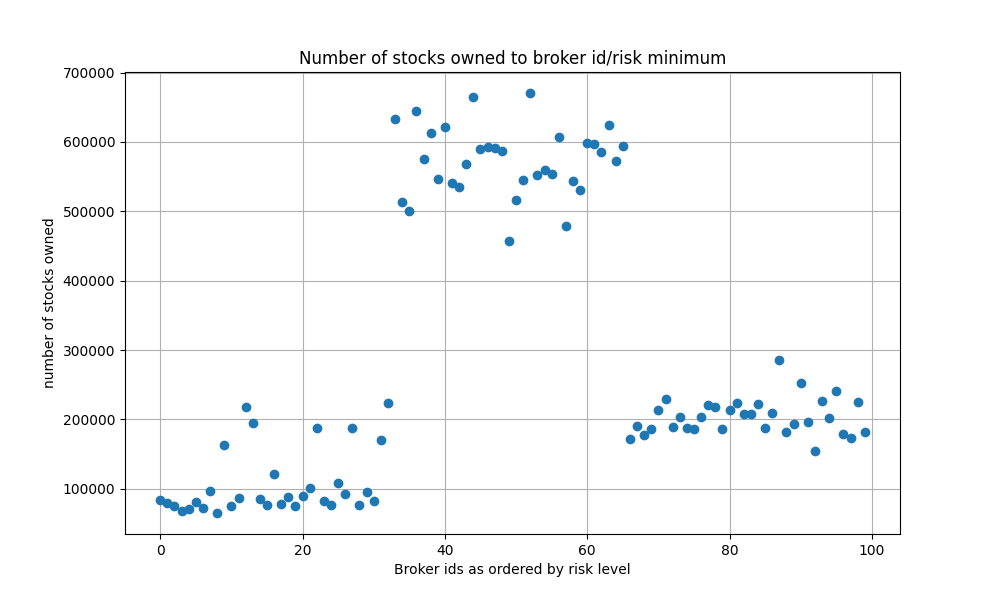
\includegraphics[width=0.4\textwidth]{stocksOwnedToBrokerIds.png}
		\caption{Total number of stocks owned by Broker Id}
		\label{totalvID}
	\end{figure}
	\FloatBarrier

	Fig \ref{uniquevID} assists in describing how the total number of stocks owned has two values. Here, the levels at which unique stocks are owned are inverted compared to Fig \ref{totalvID}. Both risk-averse and risky brokers tend to own a number of unique stocks, while those with medium risk tend to own more of the same type of stocks. The ownership of multiple stocks in different industries can be seen as less risky, as owning more individual stocks allows certain investments to fail without affecting the total as much. This is compared to a high ownership of a specific stock, which, if it goes under, results in the entire portfolio going under as well. 

	\begin{figure}[h]
		\centering
		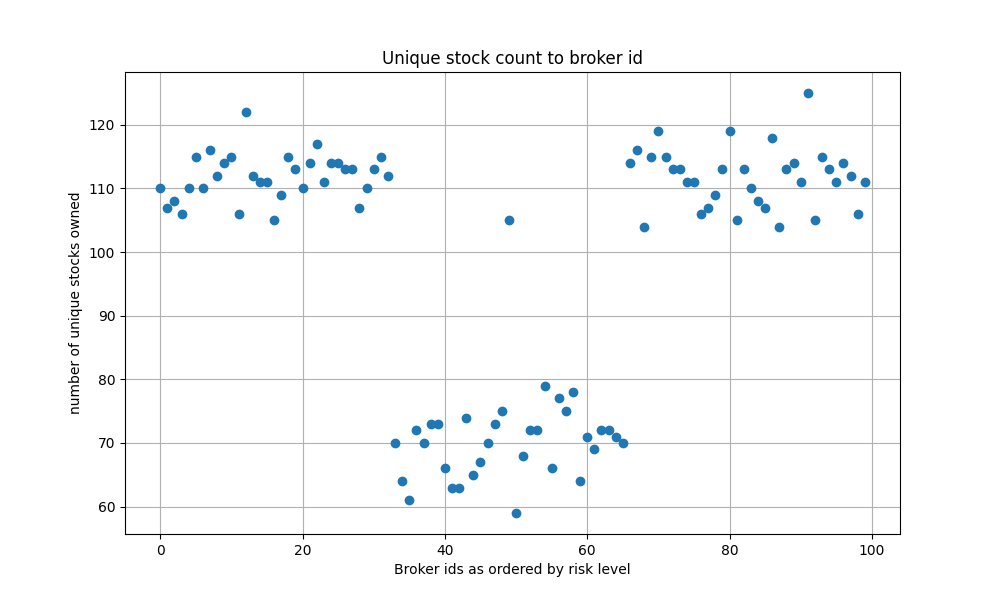
\includegraphics[width=0.4\textwidth]{uniqueStockCountToBrokerIds.png}
		\caption{Unique stocks owned by Broker Id}
		\label{uniquevID}
	\end{figure}
	\FloatBarrier

	Finally, the amount of liquid assets of each broker paints a clear picture of the differing investment strategies of low and high-risk investors. Fig \ref{liquidvID} shows that risk-averse brokers tend to keep as much as 100\% of their assets liquid, meaning they are not invested in the market. Meanwhile, medium and high-risk brokers tend to invest most of their assets into the market. These three figures illustrate the various strategies that brokers with varying levels of risk aversion employ.

	\begin{figure}[h]
		\centering
		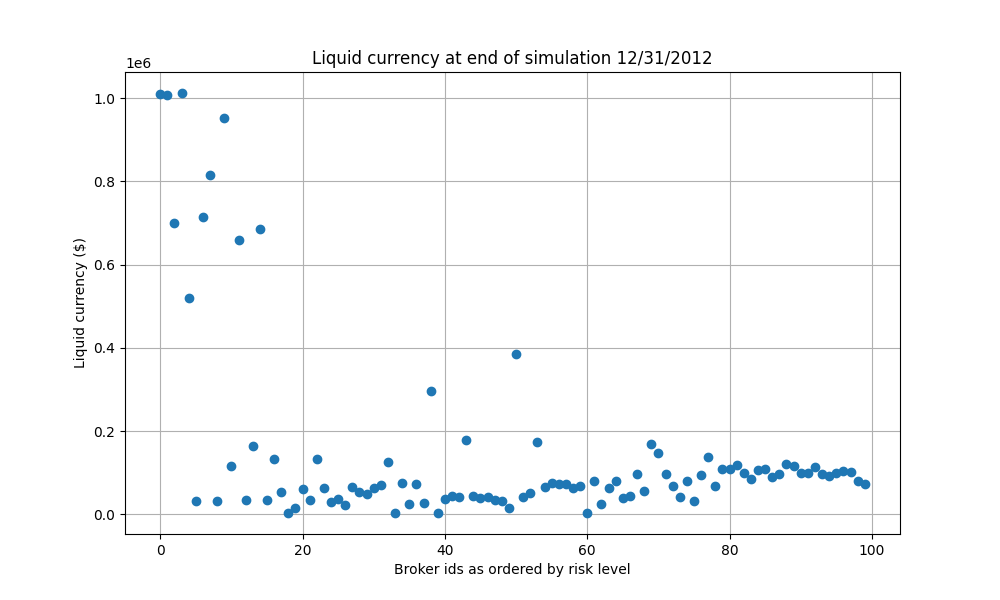
\includegraphics[width=0.4\textwidth]{liquidCurrency.png}
		\caption{Liquid currency vs Broker Id}
		\label{liquidvID}
	\end{figure}
	\FloatBarrier	

	\subsection{Market Strategies}\label{subsec:results_midpoint}
	Each strategy is followed throughout the period of 2003 to 2012, with the occurrence of the black swan event, the 2008 financial crisis, happening during this time period. Therefore, it is beneficial to analyze how different risk strategies performed with and without the black swan event to determine if certain strategies are better given antifragile thinking. Fig \ref{interimRV} shows that pre-2008, both high and medium-risk strategies outperformed low-risk strategies. However, the most risky brokers were significantly underperforming their peers. It is important to note that all brokers were able to increase their portfolio value over this time.

	\begin{figure}[h]
		\centering
		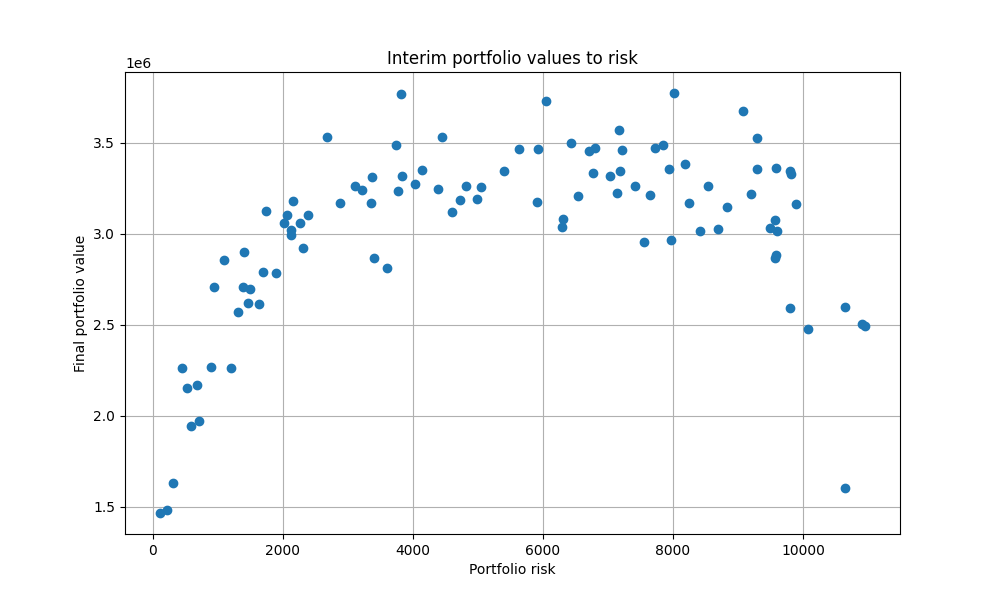
\includegraphics[width=0.4\textwidth]{interimRiskToValue.png}
		\caption{Value of Portfolios before Black Swan event}
		\label{interimRV}
	\end{figure}
	\FloatBarrier

	\subsection{Antifragile Strategies}\label{subsec:results_end}	
	
	Both Fig \ref{ts_03-12} and Fig \ref{RV} show the resultant wealth of brokers throughout the simulation. Fig \ref{ts_03-12} displays the time series of each of the portfolios. A few trends are of note. Firstly, the total wealth of the brokers' assets all appear to follow the general market trendline, and therefore all follow each other. All of the brokers experienced a significant loss due to the 2008 financial crisis; however, it is important to note that all the brokers "rode out the wave" and kept their assets. This resulted in, by 2012, the brokers regaining the wealth that they had acquired before 2008. Other brokers rebounded significantly well compared to their peers, specifically those brokers with medium risk.

	\begin{figure}[h]
		\centering
		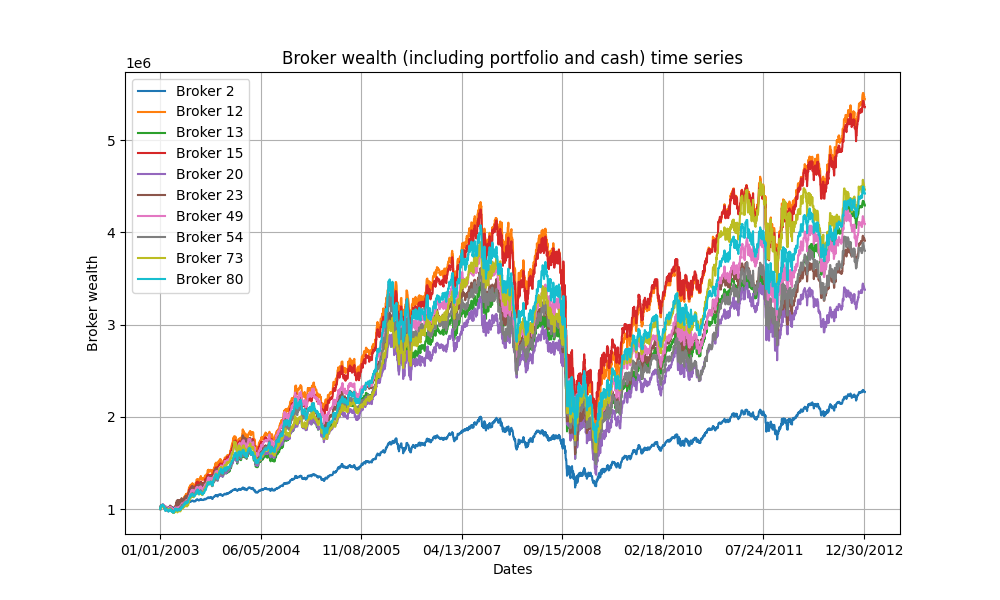
\includegraphics[width=0.4\textwidth]{timeSeriesJoint.png}
		\caption{Timeseries of Broker Wealth}
		\label{ts_03-12}
	\end{figure}
	\FloatBarrier

	As was the case for Fig \ref{interimRV}, the medium-risk brokers appeared to have acquired the most wealth. Fig \ref{RV} differs from the pre-black swan event wealth in a few key categories. First, high-risk brokers were punished significantly worse than before the black swan event. The curve in Fig \ref{RV} is very parabolic, where both the low and high-risk brokers did not acquire as much wealth as the average-risk broker. This is in comparison to Fig \ref{interimRV}, where the curve flattens and stays flat, indicating that high-risk brokers also perform well.

	\begin{figure}[h]
		\centering
		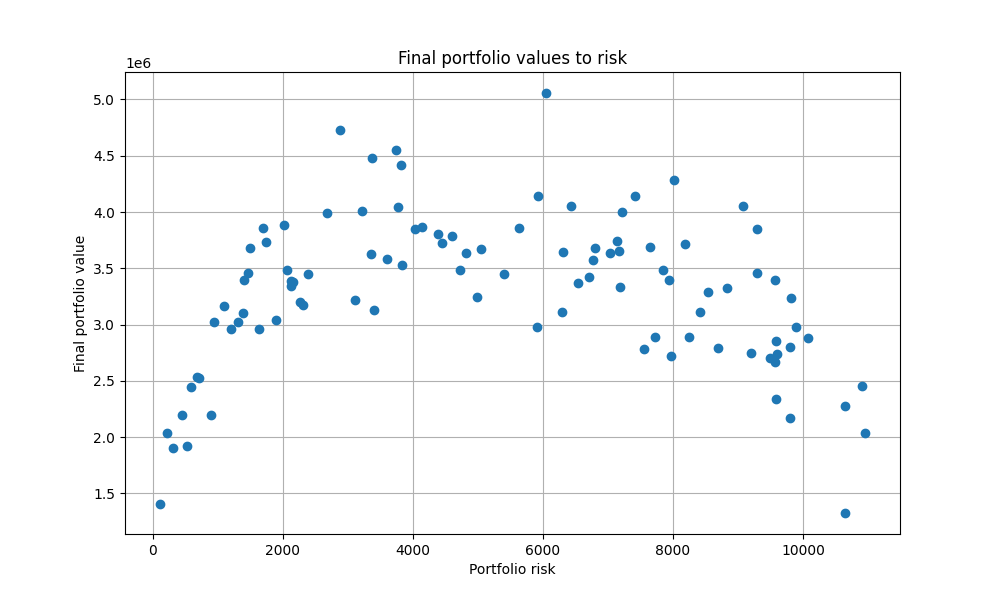
\includegraphics[width=0.4\textwidth]{valueToRisk.png}
		\caption{Value of Portfolios by Broker Id}
		\label{RV}
	\end{figure}
	\FloatBarrier
	
	Additionally, simulations were performed where once a broker accomplished their desired risk, they would stop investing. This was to simulate a real-world strategy of investing and sitting on the investment. Interestingly, brokers, although starting with the same risks as in other simulations, ended up becoming less risky by the end of the simulation. Fig \ref{stopatstable} shows that most brokers decided to become less risky, some with zero risk. This is in comparison to Fig \ref{RV}, where the distribution of risk is linear by the end of the simulation. It is also important to note that brokers "sitting on their investments" performed similarly to brokers who continuously invested after the black swan event.

	\begin{figure}[h]
		\centering
		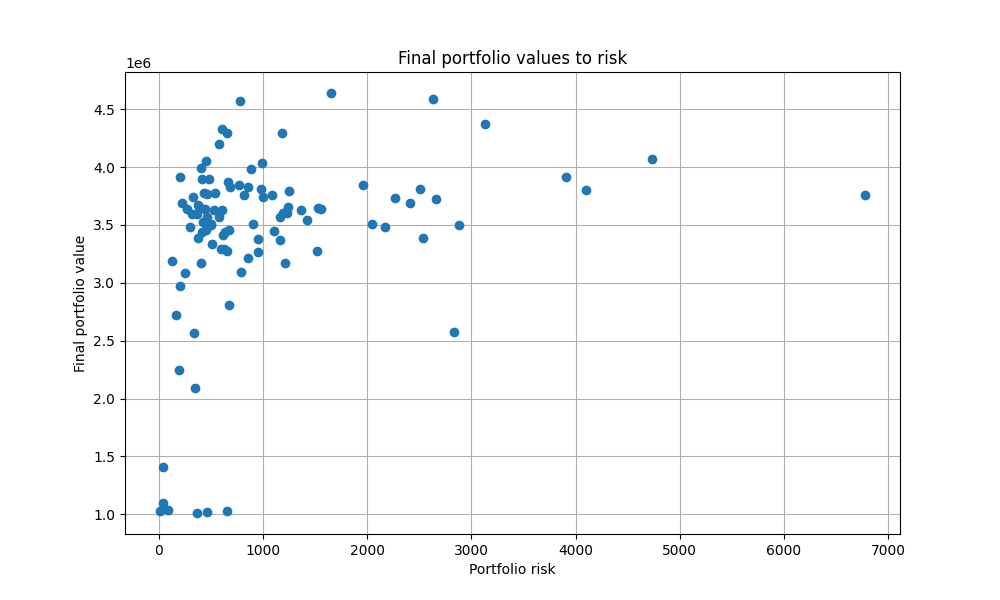
\includegraphics[width=0.4\textwidth]{valueToRisk_stopatstable.png}
		\caption{Portfolio values by risk when Brokers stop at their }
		\label{stopatstable}
	\end{figure}
	\FloatBarrier

	% here's our figure insertion template
%	\begin{figure}[h]
%		\centering
%		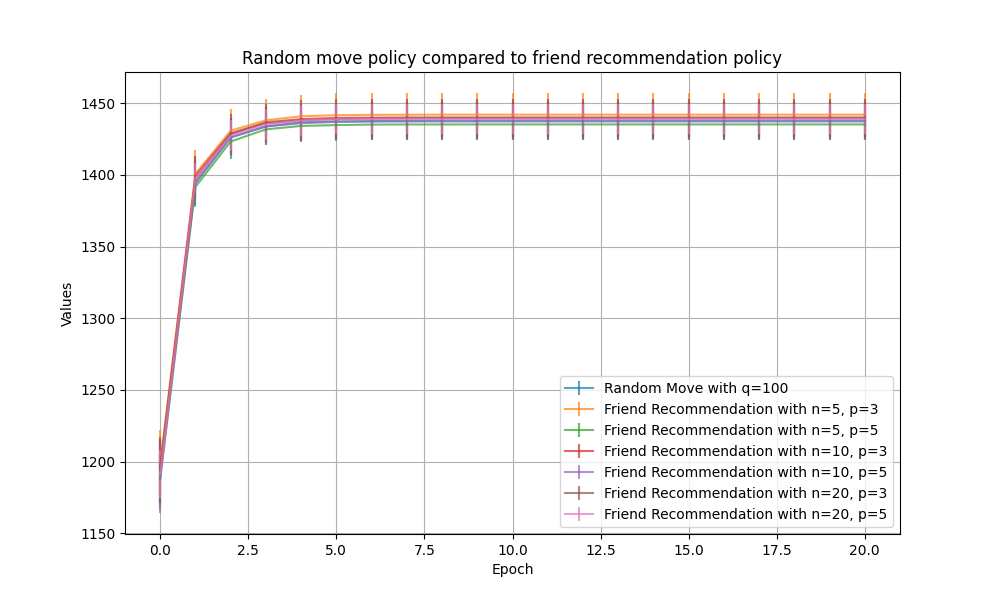
\includegraphics[width=.8\textwidth]{policies01.png}
%		\caption{Time series comparing a random move policy with the social network recommendation policy}
%		\label{p2_ts}
%	\end{figure}	
	
	
	\subsection{Influence}
	% influence results
	% Seems like influence as is feeds into risk incorrectly because the only difference between the broker's assessment is really how much of that stock they own and its value in their portfolio
	% influence would be more relevant if partial information came into play instead of just how risky the broker wanted to be
	
	\begin{figure}[h]
		\centering
		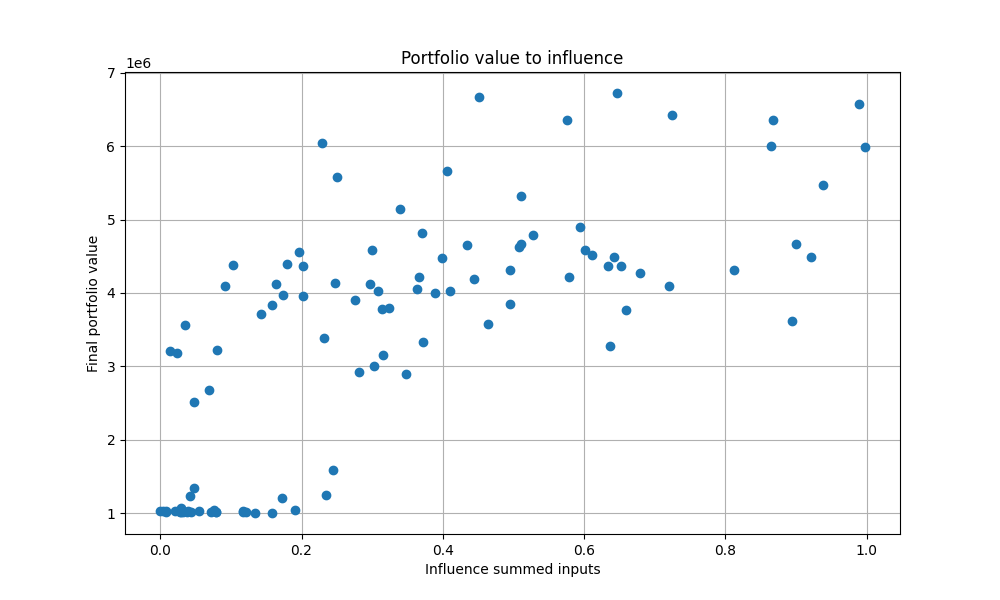
\includegraphics[width=.4\textwidth]{valueToInfluence_influence04.png}
		\caption{Plot of portfolio values to percent of decision made based on friends' recommendations on risk}
		\label{fig:value_to_influence_influencerun}
	\end{figure}	
	\FloatBarrier
	
	\begin{figure}[h]
		\centering
		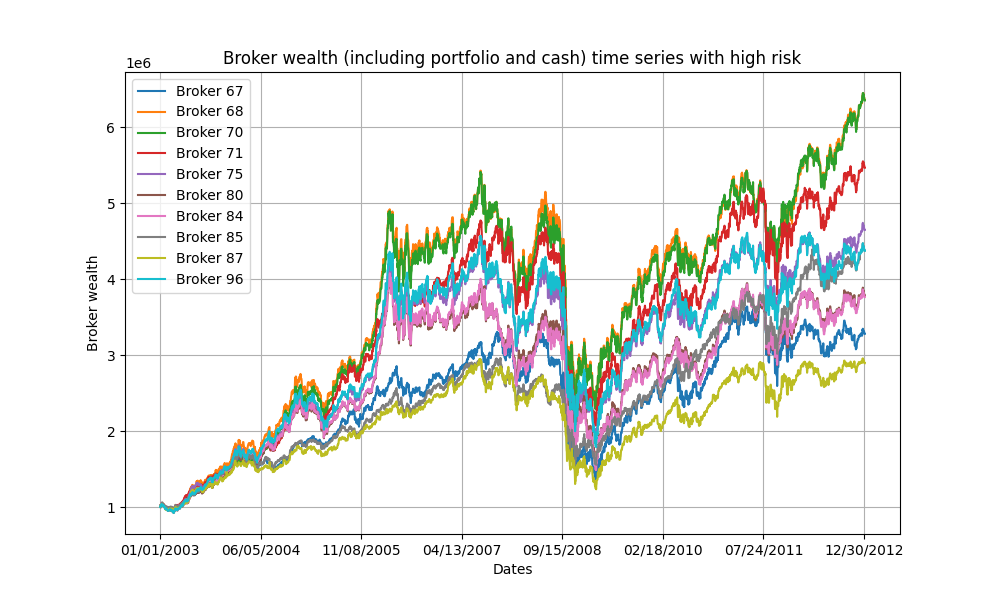
\includegraphics[width=.4\textwidth]{timeSeriesJoint_influenceRun04_HighRisk.png}
		\caption{Time series of portfolio values of brokers with high risk ordered by number of friends providing input on risk assessment for stock purchases}
		\label{fig:high_risk_influence_time_series}
	\end{figure}	
	\FloatBarrier

	\begin{figure}[h]
		\centering
		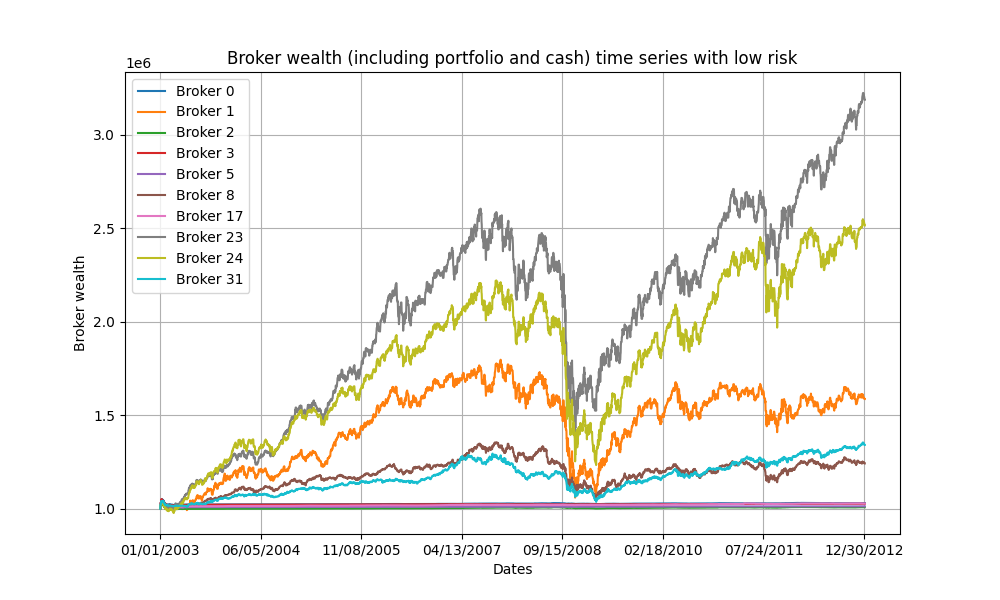
\includegraphics[width=.4\textwidth]{timeSeriesJoint_influenceRun04_LowRisk.png}
		\caption{Time series of portfolio values of brokers with low risk ordered by number of friends providing input on risk assessment for stock purchases}
		\label{fig:low_risk_influence_time_series}
	\end{figure}	
	\FloatBarrier

	The simulation examining the impact of influence assigned the brokers to either a low, medium, or high risk level. Within each group, the brokers were ordered from lowest amount of initial friends to greatest quantity, sampled from the fat-tailed distribution discussed in \ref{subsec:friends}. The plot in Figure \ref{fig:value_to_influence_influencerun} shows that allowing a large 50-100\% portion of the purchase assessment to be made with input from neighbors improves the portfolio value. While there is a wide range of values coming from a given influence, it generally improves up to around 50\% of the risk assessment being provided by friends. This is likely because taking multiple neighbors' input highlights stocks that are doing well for multiple different brokers, making the decision easier and capturing the change in value directly that the risk assessment did not capture. Further, it can be seen that this benefit of influence was consistent across the different risk levels by examining Figures \ref{fig:low_risk_influence_time_series} and  and \ref{fig:high_risk_influence_time_series}. It is notable that basing the influence connections of the network around the risk assessment provides an expansion on a single broker's understanding of the stocks behavior  but did not entirely capture the additional benefit of accessing partial information as desired.
	
	
	\section{Conclusion}\label{sec:conclusion}
	% Conclusion: Summary of accomplishments, challenges and open issues
	This project explored the value of different risk strategies in a simulated market of networked brokers with power law assumptions for risk and connectivities between brokers. It demonstrated the value of taking some input from neighbors' assessments on risk to filter which stocks are actually performing well and showed ... % highlight benefits of risk
	
	\subsection{Future Work}\label{subsec:futurework}
	Given the scope of time for the project, only limited aspects of market strategies could be explored. One open area in which limited advances were made was exploring the impact of the influence of neighbors' assessment of risk on the success of a strategy. Because all neighbors used the same information and formula, except for the accounting of their personal status, the impact of influence could be expanded. Further, the risk assessment would be modified to vary more between brokers based on partial information and stocks without full information available to better represent the real world and better account for the interconnections between stocks. \par



	\bibliographystyle{ieeetran}
	\begin{thebibliography}{99}	
		\bibitem{gabaix_powerlaws}
		X. Gabaix, “Power laws in economics: an introduction,” \textit{Journal of Economic Perspectives}, vol. 30, no. 1, pp. 185–206, Feb. 2016.
		
		\bibitem{taleb_antifragile}
		N. N. Taleb, Antifragile: Things that gain from disorder. Harlow, England: Penguin Books, 2013.
		
		\bibitem{easley_networkscrowdsmmarkets}
		D. Easley and J. Kleinberg, Networks, crowds, and markets: Reasoning about a highly connected world. Cambridge, England: Cambridge University Press, 2012.
		%- https://www.cs.cornell.edu/home/kleinber/networks-book/, particularly chapters 9-12, 17, 22
		
	
		\bibitem{hommes_complexmacroeconomics}
		C. Hommes, “Behavioral and Experimental Macroeconomics and Policy Analysis: A Complex Systems Approach,” Journal of Economic Literature, vol. 59, no. 1, pp. 149–219, Mar. 2021, doi: 10.1257/jel.20191434.
		%- https://pubs.aeaweb.org/doi/pdfplus/10.1257/jel.20191434
		
		\bibitem{tse_networkstocks}
		C. K. Tse, J. Liu, and F. C. M. Lau, “A network perspective of the stock market,” Journal of Empirical Finance, vol. 17, no. 4, pp. 659–667, Sep. 2010, doi: 10.1016/j.jempfin.2010.04.008.
		%- https://www.sciencedirect.com/science/article/pii/S0927539810000368
		
		\bibitem{kulmann_marketscomplexsystems}
		M. Kuhlmann, "Explaining financial markets in terms of complex systems," \textit{Philosphy of Science}, vol. 81, no. 5, pp. 1117-1130, Dec. 2014. %doi: 10.1086/677699.
		
		\bibitem{dimaggio_relevancebrokernetworks}
		M. Di Maggio, F. Franzoni, A. Kermani, and C. Sommavilla, "The relevance of broker networks for information diffusion in the stock market," \textit{Journal of Financial Economics}, vol. 134, no. 2, pp. 419-446, Nov. 2019. %doi: 10.1016/j.jfineco.2019.04.002. 
		
		
		\bibitem{gai_contagion}
		P. Gai and S. Kapadia, "Contagion in financial networks," \textit{Proceedings of the Royal Society}, vol. 466, no. 2120, pp. 2401–2423, Aug. 2010.
		
		\bibitem{liu_networkperspective}
		C. K. Tse, J. Liu, and F. C. M. Lau, “A network perspective of the stock market,” \textit{Journal of Empirical Finance}, vol. 17, no. 4, pp. 659–667, Sep. 2010. % doi: 10.1016/j.jempfin.2010.04.008.
		
		\bibitem{li_correlation}
		G. Li, A. Zhang, Q. Zhang, D. Wu, and C. Zhan, “Pearson correlation coefficient-based performance enhancement of broad learning system for stock price prediction,” \textit{IEEE Transactions on Circuits and Systems II: Express Briefs}, vol. 69, no. 5, pp. 2413–2417, May 2022. %, doi: 10.1109/TCSII.2022.3160266.
		
		\bibitem{fiedor_networksmutualinformationrate}
		P. Fiedor, “Networks in financial markets based on the mutual information rate,” \textit{Physical Review E}, vol. 89, no. 5, May 2014. % doi: 10.1103/PhysRevE.89.052801.
		
		\bibitem{cooper_realinvestmentandrisk}
		I. Cooper and R. Priestley. "Real investment and risk dynamics," \textit{Journal of Financial Economics}, vol. 101, no. 1, pp. 182-205, July 2011.
		
		\bibitem{lansing_riskaversion}
		K. J. Lansing and S. F. LeRoy, “Risk aversion, investor information and stock market volatility,” \textit{European Economic Review}, vol. 70, pp. 88-107, July 2014. 
		
		\bibitem{risktolerance}
		J. E. Corter and Y. J. Chen, “Do investment risk tolerance attitudes predict portfolio risk?,” \textit{Journal of Business and Psychology}, vol. 20, no. 3, pp. 369-381, 2006.
		
		\bibitem{harmon_economicinterdependence}
		D. Harmon, B. Stacey, Y. Bar-Yam, and Y. Bar-Yam, "Networks of economic market interdependence and systemic risk," New England Complex Systems Institute, Cambridge, MA, Tech. Report 1011.3707, Mar. 2009.
		
		\bibitem{baydelli_hierarchicalmarket}
		Y. Y. Baydilli, S. Bayir, and I. Tuker, “A hierarchical view of a national stock market as a complex network,” \textit{Economic Computation \& Economic Cybernetics Studies \& Research}, vol. 51, no. 1, pp. 205–222, Jan. 2017.
		
	\end{thebibliography}

		

%	\thanks{This work was contributed by }

\end{document}